% Generated by code/needham.py -- do not edit by hand.
\definecolor{qocA}{rgb}{0.00,0.45,0.70}
\definecolor{qocB}{rgb}{0.90,0.60,0.00}
\definecolor{qocC}{rgb}{0.00,0.62,0.45}
\definecolor{qocD}{rgb}{0.80,0.40,0.00}
\definecolor{qocE}{rgb}{0.80,0.60,0.70}
\definecolor{qocF}{rgb}{0.35,0.70,0.90}
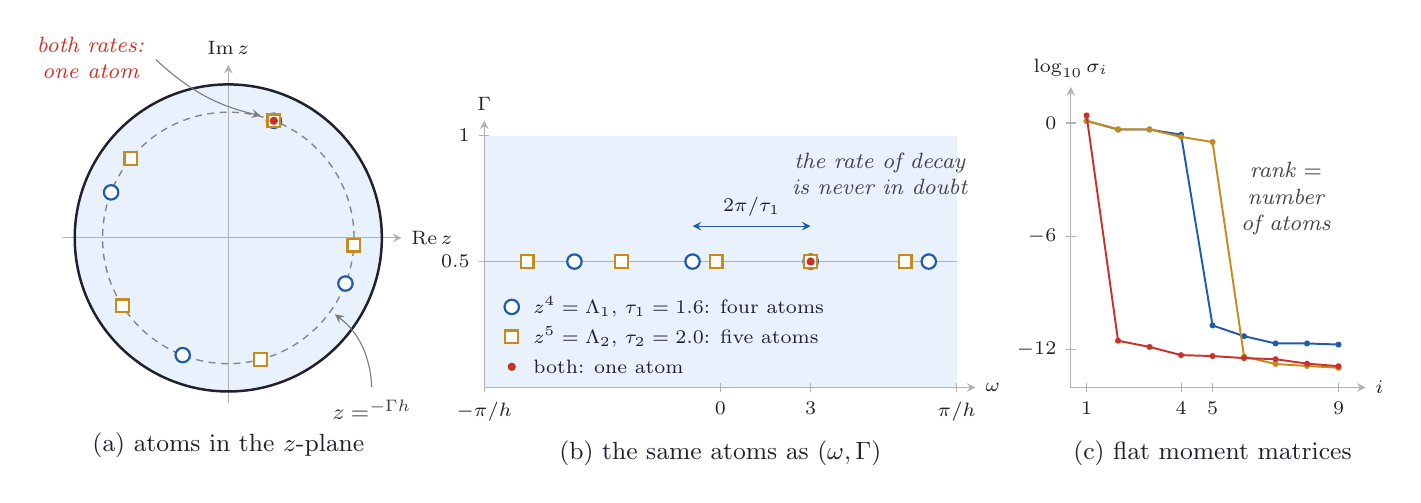
\begin{tikzpicture}[ink/.style={line width=0.9pt, ndInk}, faint/.style={line width=0.4pt, ndInk!35}, dashedink/.style={line width=0.5pt, ndInk!55, dash pattern=on 2.5pt off 2pt}, vec/.style={->, >=stealth, line width=1.2pt}, note/.style={font=\footnotesize\itshape, text=ndInk!85, align=center}, pointer/.style={->, >=stealth, line width=0.4pt, ndInk!60, shorten >=2pt, shorten <=1pt}, dot/.style={circle, fill=ndInk, inner sep=0pt, minimum size=3.4pt}, wash/.style={fill=ndSky, fill opacity=0.55}, every node/.style={text=ndInk}]
\definecolor{ndInk}{rgb}{0.13,0.13,0.18}
\definecolor{ndPaper}{rgb}{0.99,0.96,0.88}
\definecolor{ndSky}{rgb}{0.84,0.91,0.98}
\definecolor{ndRose}{rgb}{0.98,0.86,0.84}
\definecolor{ndBlue}{rgb}{0.13,0.36,0.66}
\definecolor{ndRed}{rgb}{0.78,0.20,0.16}
\definecolor{ndGold}{rgb}{0.88,0.62,0.10}
\definecolor{ndGreen}{rgb}{0.18,0.52,0.30}
\fill[ndSky!55] (2.300,2.750) circle (1.950);
\draw[faint, ->, >=stealth] (0.200,2.750) -- (4.500,2.750) node[right, text=ndInk] {\scriptsize $\mathrm{Re}\,z$};
\draw[faint, ->, >=stealth] (2.300,0.650) -- (2.300,4.950) node[above, text=ndInk] {\scriptsize $\mathrm{Im}\,z$};
\draw[ink] (2.300,2.750) circle (1.950);
\draw[dashedink] (2.300,2.750) circle (1.597);
\draw[ndBlue, line width=0.8pt, fill=white] (1.721,1.262) circle (2.60pt);
\draw[ndBlue, line width=0.8pt, fill=white] (3.788,2.171) circle (2.60pt);
\draw[ndBlue, line width=0.8pt, fill=white] (2.879,4.238) circle (2.60pt);
\draw[ndBlue, line width=0.8pt, fill=white] (0.812,3.329) circle (2.60pt);
\draw[ndGold!85!ndInk, line width=0.8pt, fill=white] (0.876,1.805) rectangle (1.038,1.967);
\draw[ndGold!85!ndInk, line width=0.8pt, fill=white] (2.626,1.125) rectangle (2.787,1.287);
\draw[ndGold!85!ndInk, line width=0.8pt, fill=white] (3.813,2.579) rectangle (3.975,2.740);
\draw[ndGold!85!ndInk, line width=0.8pt, fill=white] (2.798,4.157) rectangle (2.959,4.319);
\draw[ndGold!85!ndInk, line width=0.8pt, fill=white] (0.983,3.679) rectangle (1.144,3.841);
\fill[ndRed] (2.879,4.238) circle (1.5pt);
\node[note, anchor=north west] (ra) at (3.500,0.820) {$\abs z=\ee^{-\Gamma h}$};
\draw[pointer] (ra.north) to[bend right=25] (3.599,1.822);
\node[note, anchor=south, text=ndRed] (tr) at (0.550,4.650) {both rates:\\ one atom};
\draw[pointer] (tr.east) to[bend right=15] (2.779,4.288);
\node[font=\small, anchor=north] at (2.300,0.400) {(a) atoms in the $z$-plane};
\fill[ndSky!55] (5.550,0.850) rectangle (11.550,4.050);
\draw[faint, ->, >=stealth] (5.550,0.850) -- (11.790,0.850) node[right, text=ndInk] {{\scriptsize $\omega$}};
\draw[faint, ->, >=stealth] (5.550,0.850) -- (5.550,4.242) node[above, text=ndInk] {{\scriptsize $\Gamma$}};
\draw[faint] (5.550,0.910) -- (5.550,0.790) node[below, font=\scriptsize, text=ndInk] {$-\pi/h$};
\draw[faint] (8.550,0.910) -- (8.550,0.790) node[below, font=\scriptsize, text=ndInk] {$0$};
\draw[faint] (9.696,0.910) -- (9.696,0.790) node[below, font=\scriptsize, text=ndInk] {$3$};
\draw[faint] (11.550,0.910) -- (11.550,0.790) node[below, font=\scriptsize, text=ndInk] {$\pi/h$};
\draw[faint] (5.610,2.450) -- (5.490,2.450) node[left, font=\scriptsize, text=ndInk] {$0.5$};
\draw[faint] (5.610,4.050) -- (5.490,4.050) node[left, font=\scriptsize, text=ndInk] {$1$};
\draw[faint] (5.550,2.450) -- (11.550,2.450);
\draw[ndBlue, line width=0.8pt, fill=white] (6.696,2.450) circle (2.60pt);
\draw[ndBlue, line width=0.8pt, fill=white] (8.196,2.450) circle (2.60pt);
\draw[ndBlue, line width=0.8pt, fill=white] (9.696,2.450) circle (2.60pt);
\draw[ndBlue, line width=0.8pt, fill=white] (11.196,2.450) circle (2.60pt);
\draw[ndGold!85!ndInk, line width=0.8pt, fill=white] (6.015,2.369) rectangle (6.177,2.531);
\draw[ndGold!85!ndInk, line width=0.8pt, fill=white] (7.215,2.369) rectangle (7.377,2.531);
\draw[ndGold!85!ndInk, line width=0.8pt, fill=white] (8.415,2.369) rectangle (8.577,2.531);
\draw[ndGold!85!ndInk, line width=0.8pt, fill=white] (9.615,2.369) rectangle (9.777,2.531);
\draw[ndGold!85!ndInk, line width=0.8pt, fill=white] (10.815,2.369) rectangle (10.977,2.531);
\fill[ndRed] (9.696,2.450) circle (1.5pt);
\draw[ndBlue, line width=0.8pt, fill=white] (5.900,1.874) circle (2.60pt);
\node[font=\scriptsize, anchor=west] at (6.050,1.874) {$z^4=\Lambda_1$, $\tau_1=1.6$: four atoms};
\draw[ndGold!85!ndInk, line width=0.8pt, fill=white] (5.819,1.413) rectangle (5.981,1.575);
\node[font=\scriptsize, anchor=west] at (6.050,1.494) {$z^5=\Lambda_2$, $\tau_2=2.0$: five atoms};
\fill[ndRed] (5.900,1.114) circle (1.5pt);
\node[font=\scriptsize, anchor=west] at (6.050,1.114) {both: one atom};
\draw[<->, >=stealth, line width=0.4pt, ndBlue] (8.196,2.900) -- (9.696,2.900) node[midway, above, font=\scriptsize] {$2\pi/\tau_1$};
\node[note, anchor=north] at (10.574,3.954) {the rate of decay\\ is never in doubt};
\node[font=\small, anchor=north] at (8.550,0.300) {(b) the same atoms as $(\omega,\Gamma)$};
\draw[faint, ->, >=stealth] (13.000,0.850) -- (16.744,0.850) node[right, text=ndInk] {{\scriptsize $i$}};
\draw[faint, ->, >=stealth] (13.000,0.850) -- (13.000,4.666) node[above, text=ndInk] {{\scriptsize $\log_{10}\sigma_i$}};
\draw[faint] (13.200,0.910) -- (13.200,0.790) node[below, font=\scriptsize, text=ndInk] {$1$};
\draw[faint] (14.400,0.910) -- (14.400,0.790) node[below, font=\scriptsize, text=ndInk] {$4$};
\draw[faint] (14.800,0.910) -- (14.800,0.790) node[below, font=\scriptsize, text=ndInk] {$5$};
\draw[faint] (16.400,0.910) -- (16.400,0.790) node[below, font=\scriptsize, text=ndInk] {$9$};
\draw[faint] (13.060,4.210) -- (12.940,4.210) node[left, font=\scriptsize, text=ndInk] {$0$};
\draw[faint] (13.060,2.770) -- (12.940,2.770) node[left, font=\scriptsize, text=ndInk] {$-6$};
\draw[faint] (13.060,1.330) -- (12.940,1.330) node[left, font=\scriptsize, text=ndInk] {$-12$};
\draw[line width=0.7pt, ndBlue] (13.200,4.237) -- (13.600,4.127) -- (14.000,4.127) -- (14.400,4.061) -- (14.800,1.639) -- (15.200,1.502) -- (15.600,1.410) -- (16.000,1.410) -- (16.400,1.396);
\fill[ndBlue] (13.200,4.237) circle (1.1pt);
\fill[ndBlue] (13.600,4.127) circle (1.1pt);
\fill[ndBlue] (14.000,4.127) circle (1.1pt);
\fill[ndBlue] (14.400,4.061) circle (1.1pt);
\fill[ndBlue] (14.800,1.639) circle (1.1pt);
\fill[ndBlue] (15.200,1.502) circle (1.1pt);
\fill[ndBlue] (15.600,1.410) circle (1.1pt);
\fill[ndBlue] (16.000,1.410) circle (1.1pt);
\fill[ndBlue] (16.400,1.396) circle (1.1pt);
\draw[line width=0.7pt, ndGold!85!ndInk] (13.200,4.236) -- (13.600,4.130) -- (14.000,4.129) -- (14.400,4.033) -- (14.800,3.968) -- (15.200,1.244) -- (15.600,1.149) -- (16.000,1.124) -- (16.400,1.101);
\fill[ndGold!85!ndInk] (13.200,4.236) circle (1.1pt);
\fill[ndGold!85!ndInk] (13.600,4.130) circle (1.1pt);
\fill[ndGold!85!ndInk] (14.000,4.129) circle (1.1pt);
\fill[ndGold!85!ndInk] (14.400,4.033) circle (1.1pt);
\fill[ndGold!85!ndInk] (14.800,3.968) circle (1.1pt);
\fill[ndGold!85!ndInk] (15.200,1.244) circle (1.1pt);
\fill[ndGold!85!ndInk] (15.600,1.149) circle (1.1pt);
\fill[ndGold!85!ndInk] (16.000,1.124) circle (1.1pt);
\fill[ndGold!85!ndInk] (16.400,1.101) circle (1.1pt);
\draw[line width=0.7pt, ndRed] (13.200,4.306) -- (13.600,1.445) -- (14.000,1.366) -- (14.400,1.262) -- (14.800,1.250) -- (15.200,1.224) -- (15.600,1.210) -- (16.000,1.154) -- (16.400,1.121);
\fill[ndRed] (13.200,4.306) circle (1.1pt);
\fill[ndRed] (13.600,1.445) circle (1.1pt);
\fill[ndRed] (14.000,1.366) circle (1.1pt);
\fill[ndRed] (14.400,1.262) circle (1.1pt);
\fill[ndRed] (14.800,1.250) circle (1.1pt);
\fill[ndRed] (15.200,1.224) circle (1.1pt);
\fill[ndRed] (15.600,1.210) circle (1.1pt);
\fill[ndRed] (16.000,1.154) circle (1.1pt);
\fill[ndRed] (16.400,1.121) circle (1.1pt);
\node[note, anchor=west] at (15.040,3.250) {rank $=$\\ number\\ of atoms};
\node[font=\small, anchor=north] at (14.800,0.300) {(c) flat moment matrices};
\end{tikzpicture}
